\subsection{Task 1: Degree distribution}

\subsubsection{Description}
We conduct 5 experiments on large scale graph data(all with more than 1 million nodes). Following are the plots of each dataset, Figure \ref{t1:wiki} shows the in degree and out degree out Wikitalk. Figure \ref{t1:ca}(a) is Roadnet-Ca. Figure \ref{t1:ca}(b) is Roadnet-PA. Figure \ref{t1:tx}(a) is Roadnet-TX. Figure \ref{t1:tx}(b) is Youtube. 

\subsubsection{Plots}

\begin{figure}[hf]
\begin{center}
\begin{tabular}{cc}
     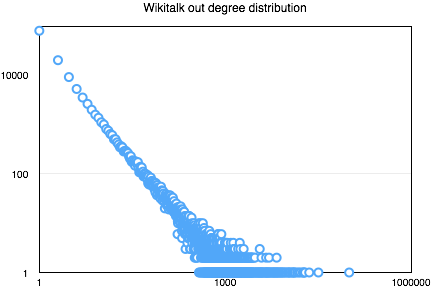
\includegraphics[width=0.4\textwidth]{FIG/t1_wiki_in.png} &
     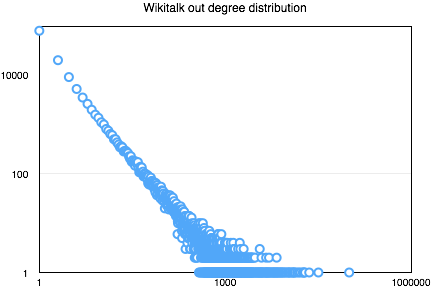
\includegraphics[width=0.4\textwidth]{FIG/t1_wiki_out.png} \\
    (a) & (b) 
\end{tabular}
\caption{In degree distribution (a) and out degree distribution (b) of Wikitalk}
\label{t1:wiki}
\end{center}
\end{figure}

\begin{figure}[hf]
\begin{center}
\begin{tabular}{cc}
     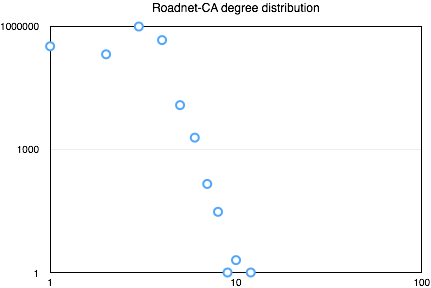
\includegraphics[width=0.4\textwidth]{FIG/t1_ca.png} &      
     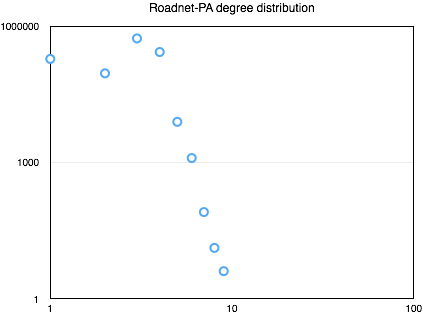
\includegraphics[width=0.4\textwidth]{FIG/t1_pa.png} \\
     (a) & (b)
\end{tabular}
\caption{Degree distribution of (a) Roadnet-CA, (b) Roadnet-PA}
\label{t1:ca}
\end{center}
\end{figure}

\begin{figure}[hf]
\begin{center}
\begin{tabular}{cc}
     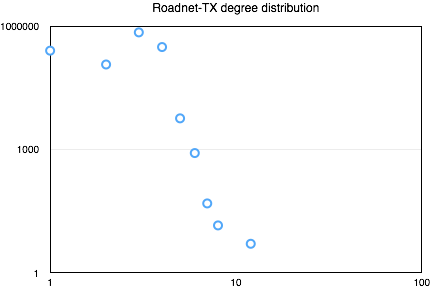
\includegraphics[width=0.4\textwidth]{FIG/t1_tx.png} & 
     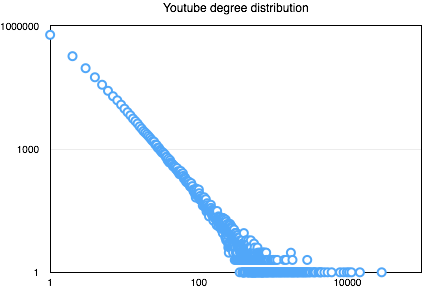
\includegraphics[width=0.4\textwidth]{FIG/t1_youtube.png} \\
     (a) & (b)
\end{tabular}
\caption{Degree distribution of (a) Roadnet-TX, and (b) Youtube}
\label{t1:tx}
\end{center}
\end{figure}

\subsubsection{Observation}
FILL in later. 